%% Para compilar o programa, use pdflatex
%% Opcoes:
%%
%% Cursos:
%% cic: Bacharelado em Ciência da Computação
%% tsi: Técnologo em Sistemas para Internet
\documentclass[tsi]{ifbclass/ifbclass}

\address{BRASÍLIA}

\title{Título do Trabalho}

\date{2018}

\author{Nome completo do Autor}
\adviser{Nome completo do Orientador}

\membroum[a]{Dr.ª Primeira Membro da Banca}
\membrodois{Dr. Segundo Membro da Banca}
\membrotres[a]{Dr.ª Terceira Membro da Banca}
%\membroquatro[a]{Dr.ª Quarta Membro da Banca}

%\coadviser{Nome completo do co-orientador (se existir)} %TODO: nao suportado

% Macros (Se necessario, defina suas proprias aqui)
\def\x{\checkmark}
%\let\lstlistoflistings\origlstoflistings
  \begin{document}

\frontmatter

\frontpage

\presentationpage

% Quando a biblioteca preparar a ficha catalografica, insira-a aqui
% Antes da defesa do trabalho, crie uma ficha falsa
\begin{fichacatalografica}
  \FakeFichaCatalografica
%     \includepdf{fig_ficha_catalografica.pdf} % crie o arquivo come esse nome e descomente essa linha
\end{fichacatalografica}

\banca

%Comente/Remova todo o conteudo entre \begin{dedicatory} e \end{dedicatory} para remover.
\begin{dedicatory} %OPCIONAL
Dedico este trabalho à minha família.
\end{dedicatory}
  
\acknowledgements %OPCIONAL Comente a linha abaixo para remover.
Agradeço ao meu orientador Prof. Dr. Nome do Orientador, pela sabedoria com que me guiou nesta trajetória.

Aos meus colegas de sala.

A Secretaria do Curso, pela cooperação.

Gostaria de deixar registrado também, o meu reconhecimento à minha família, pois acredito que sem o apoio deles seria muito difícil vencer esse desafio. 

Enfim, a todos os que por algum motivo contribuíram para a realização desta pesquisa.


%Novamente, comente todo conteudo entre {epigraph} para remover
\begin{epigraph}[]{Nome do autor} %OPCIONAL
Elemento opcional.

Espaço destinado à epígrafe (elemento opcional). Nesta folha, o autor usa uma citação, seguida de indicação de autoria e ano, relacionada com a matéria tratada no corpo do trabalho.
\end{epigraph}

\resumo
% Escreva seu resumo no arquivo resumo.tex
{\parindent0pt
  SOBRENOME, Prenome do Autor do Trabalho. Título do trabalho: subtítulo (se houver).  2018. 65 f. 
Trabalho de Conclusão de Curso (Graduação) – Tecnólogo em Sistemas para Internet. 
Instituto Federal de Brasília – Campus Brasília. Brasília/DF, 2018.
\vspace{1cm}

Elemento obrigatório, constituído de uma sequência de frases concisas e objetivas,
fornecendo uma visão rápida e clara do conteúdo do estudo. O texto deverá conter no
máximo 500 palavras e ser antecedido pela referência do estudo, com exceção do resumo
inserido no próprio documento. Também, não deve conter citações. O resumo deve ser redigido
em parágrafo único, espaçamento simples e seguido das palavras representativas do conteúdo
do estudo, isto é, palavras-chave, em número de três a cinco, separadas entre si por ponto e
finalizadas também por ponto. Usar o verbo na terceira pessoa do singular, com linguagem
impessoal (pronome SE), bem como fazer uso, preferencialmente, da voz ativa.

\begin{keywords}
Primeira palavra. Segunda palavra. Terceira palavra. Quarta palavra. Quinta-palavra.
\end{keywords}

}
  
\abstract
% Escreva seu abstract em ingles no arquivo abstract.tex
{\parindent0pt
  SOBRENOME, Prenome do Autor do Trabalho. Título do trabalho: subtítulo (se houver).  2018. 65 f. 
Trabalho de Conclusão de Curso (Graduação) – Tecnólogo em Sistemas para Internet. 
Instituto Federal de Brasília – Campus Brasília. Brasília/DF, 2018.
\vspace{1cm}

Elemento obrigatório, constituído de uma sequência de frases concisas e objetivas,
fornecendo uma visão rápida e clara do conteúdo do estudo. O texto deverá conter no
máximo 500 palavras e ser antecedido pela referência do estudo, com exceção do resumo
inserido no próprio documento. Também, não deve conter citações. O resumo deve ser redigido
em parágrafo único, espaçamento simples e seguido das palavras representativas do conteúdo
do estudo, isto é, palavras-chave, em número de três a cinco, separadas entre si por ponto e
finalizadas também por ponto. Usar o verbo na terceira pessoa do singular, com linguagem
impessoal (pronome SE), bem como fazer uso, preferencialmente, da voz ativa.

\begin{keywords}
Keyword. Second keyword. Third keyword. Keyword.
\end{keywords}

}

%ATENCAO.
%Se alguma dessas listas estiver vazia no seu trabalho, comente a linha com um '%'
% Lista de figuras
\listoffigures

% Lista de algortimos
\lstlistoflistings

% Lista de tabelas
\listoftables

% Lista de acronimos
% Acronyms manual: http://linorg.usp.br/CTAN/macros/latex/contrib/acronym/acronym.pdf
\listofacronyms
\input{text/acronyms}

% Sumario
\tableofcontents

\mainmatter

%Para cada seção do seu trabalho, edite o arquivo .tex na pasta text/
\chapter{Introdução}
\label{chp:introduction}
Faça aqui, uma introdução geral da área do conhecimento à qual o tema escolhido
está ligado. 

\section{Tema}
A melhor forma de determinar o tema abordado é através de hipóteses. A hipótese
consiste em uma afirmativa que você considera verdadeira e que vai provar ou
buscar provar ao longo de seu trabalho. Outra forma é delimitando o problema em
forma de uma pergunta de partida. Apresente uma visão geral do assunto que será
abordado no trabalho.

\section{Problema}
Dedique este tópico a esclarecer o que o pretende de fato com o seu esforço de
pesquisa. Problema é a questão a ser respondida pelo trabalho, que motivou a sua
realização. É uma questão que já tomou se formou em sua mente, derivada de
teorias da área pesquisada e de sua observação sobre um fenômeno.  Normalmente
se utilizam os subitens abaixo como meios de se determinar claramente os
objetivos, o que também colabora para a delimitação do escopo do trabalho. Está
estreitamente ligado ao objetivo geral, que, normalmente, consiste em encontrar
a resposta para o problema de pesquisa.  O que você viu que é um problema que
precisa de solução? É viável? Você consegue fazer? O problema é sempre uma
dificuldade, uma lacuna.

\subsection{Objetivo geral}
É a resposta ao problema especificado acima, ou seja, aquilo que se pretende
fazer e que, depois de atingido, estará concluído o trabalho.. Alguns verbos
utilizados para determinar o objetivo geral: contribuir / facilitar / subsidiar
/ propor / clarear / permitir / agregar / compreender.

\subsection{Objetivos específicos}
Os objetivos específicos detalham os objetivos gerais através de etapas ou fases
de pesquisa. Devem ser utilizados verbos no infinitivo, assinalando as ações
propostas para alcançar o objetivo geral. Os verbos utilizados aqui são os de
ação, que serão utilizados na metodologia.


\section{Estrutura do TCC}
Neste item você vai descrever como está constituída a monografia, indicando o
que será encontrado em cada uma das sessões seguintes.

\subsection{Classificação da Pesquisa}
Neste item será apresentada a classificação da pesquisa quanto aos objetivos
(exploratória, descritiva ou explicativa); aos procedimentos (Pesquisa
bibliográfica, Pesquisa documental, Pesquisa experimental, Estudo de caso
controle, Levantamento, Estudo de caso ou Estudo de campo) e ao método de
investigação científica (qualitativa ou quantitativa).

\chapter{Conceitos gerais e revisão da literatura}
Neste capítulo deve ser proporcionado o estado da arte / referencial teórico
sobre o tema a que se refere o estudo. Um bom pesquisador não deve repetir
trabalhos já concluídos ou que já estão em andamento. Por isso esta sessão é
onde o autor demonstra até onde vai a pesquisa atual no campo de estudos em
questão e estabelece as bases sobre as quais desenvolverá o estudo proposto. A
seguir são mostrados alguns exemplos de como deve-se inserir as figuras e
tabelas. A Figura \ref{fig:exemplo} mostra um exemplo de como inserir uma
figura no texto. A Tabela \ref{tb:exemplo} mostra o exemplo de como uma tabela
deve ser inserida.  Voce pode referenciar capítulos e seções adicionando labels
à elas. Por exemplo, descrevemos a introdução no Capítulo
\ref{chp:introduction}.

\begin{figure}[!htb]
    \centering
    \caption{Exemplo de como inserir Figura}
    
\includegraphics[width=0.45\textwidth]{images/figura.png}
    \label{fig:exemplo}
\end{figure}

%Voce pode forcar a troca de pagina da seguinte forma:
\newpage

\begin{figure}[!htb]
    \centering
    \caption{Exemplo de como inserir Figura retirado de um site - Arduino Uno}
    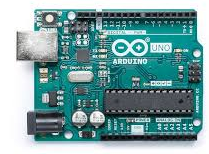
\includegraphics[width=0.35\textwidth]{images/uno.png}

    {\footnotesize Fonte: Página oficial do Arduino\protect\footnotemark}
    \label{fig:arduino_uno}
\end{figure}
\footnotetext{Disponível em: <https://www.arduino.cc/en/Main/ArduinoBoardUno>. Acesso em ago. 1999.}

%Altere o numero junto ao 'width' para acertar o tamanho da figura. Coloque
%numeros maior que 0 e até 1

\begin{table}[htb]
\caption{Modelo de como as tabelas devem ser inseridas no texto}
\label{tb:exemplo}
\centering
\begin{tabular}{|l|c|r|r|} %left, center, right. Você pode mudar isso
\hline
Índice  & Coluna 1 & Coluna 2 & Coluna 3 \\
\hline
Linha 1 &          &          &          \\
Linha 2 &          &          &          \\
Linha 3 &          &          &          \\
\hline
\end{tabular}
\end{table}
%Para manter a sanidade, recomenda-se deixar sempre os '&' alinhados em todas
%as linhas e colunas

\chapter{Metodologia}

Aqui conterão os métodos e procedimentos adotados no desenvolvimento do
trabalho. Esta é uma das sessões mais importantes pois demonstra o poder
científico que foi utilizado para a pesquisa. Sem uma boa metodologia a
pesquisa pode perder a validade. O pesquisador deve utilizar métodos ou
técnicas aceitas pela comunidade científica na busca de provar suas hipóteses.

A metodologia escolhida deve ser aquela que mais se adéqua ao seu objeto de
estudo e à abordagem aplicada. Há dois métodos principais: 1) quantitativo, que
é o uso de instrumental estatístico, de dados numéricos; e 2) qualitativo, que
se caracteriza pela qualificação dos dados coletados, durante a análise do
problema.

\section{Uma seção}
Texto.

\section{Uma outra seção}
Texto.

\chapter{Apresentação e Análise dos Resultados}

Toda pesquisa deve apresentar uma análise sobre a investigação que foi
realizada através da metodologia que foi aplicada. Nesta sessão é interessante
inserir tabelas, gráficos, imagens que mostrem os resultados, análise de dados
coletados, etc.

É interessante que nessa sessão o autor compare os seus resultados com os
resultados de outros trabalhos existentes. Essa comparação aumenta a qualidade
do trabalho e demonstra a relevância do mesmo. 

\chapter{Conclusões e Trabalhos Futuros}

A conclusão deve conter os principais aspectos e contribuições de forma a
finalizar o trabalho apresentado. Deve-se apresentar o que era esperado do
trabalho através dos objetivos inseridos inicialmente e mostrar o que foi
conseguido.

Não deve-se inserir um novo assunto na conclusão. Aqui o autor apresentará as
próprias impressões sobre o trabalho efetuado.

É importante também que sejam identificadas limitações e problemas que surgiram
durante o desenvolvimento do trabalho e quais as consequências do mesmo.

Os trabalhos futuros devem conter oportunidades de expansão do trabalho
apresentado, bem como, novos projetos que puderam ser vislumbrados a partir do
desenvolvimento do trabalho


% Referencias

\begin{references}
  \bibliography{bib/references}
\end{references}

% Apendice

\theappendix
\include{appendix/mapping-study}

\end{document}
